%!TEX program = xelatex
\documentclass{article}
\usepackage{LaTeX-Submodule/template}

% Additional packages & macros

% Header and footer
\newcommand{\unitName}{Programming Principals}
\newcommand{\unitTime}{Semester 1, 2022}
\newcommand{\unitCoordinator}{Dr Alan Woodley}
\newcommand{\documentAuthors}{\textsc{Tarang Janawalkar}}

\fancyhead[L]{\unitName}
\fancyhead[R]{\leftmark}
\fancyfoot[C]{\thepage}

% Copyright
\usepackage[
    type={CC},
    modifier={by-nc-sa},
    version={4.0},
    imagewidth={5em},
    hyphenation={raggedright}
]{doclicense}

\date{}

\begin{document}
%
\begin{titlepage}
    \vspace*{\fill}
    \begin{center}
        \LARGE{\textbf{\unitName}} \\[0.1in]
        \normalsize{\unitTime} \\[0.2in]
        \normalsize\textit{\unitCoordinator} \\[0.2in]
        \documentAuthors
    \end{center}
    \vspace*{\fill}
    \doclicenseThis
    \thispagestyle{empty}
\end{titlepage}
\newpage
%
\tableofcontents
\newpage
%
\lstset{language=[Sharp]C}
\lstset{morekeywords={with,is,as}}
\section{Programming}
\begin{definition}
    Programming is the process of designing and building an executable
    computer program to accomplish a specific computing result or to
    perform a specific task.
\end{definition}
Programming involves:
\begin{enumerate}
    \item Analysis
    \item Design
    \item Implementation
    \item Testing
\end{enumerate}
\subsection{Analysis}
\begin{itemize}
    \item What is the problem?
    \item What data is involved --- input, output?
    \item What is the relationship between input and output?
    \item What other constraints?
\end{itemize}
\subsection{Design}
\begin{itemize}
    \item Specify modules that need to be created to implement the solution.
    \item Module --- group of closely related functions and data they need to do their job
    \item Which parts of the problem are closely related? They probably belong together in a module.
    \item How do modules fit together and communicate?
    \item How can I test each of these modules to be sure they behave as desired?
    \item How can I test the complete system to be sure it behaves as desired?
\end{itemize}
\subsection{Implementation}
\begin{itemize}
    \item Create working software to "do" each part of the design
    \item Select suitable algorithms and data structures to do each required item of functionality
    \item Write code to implement the algorithms and data structures
\end{itemize}
\subsection{Testing}
\begin{itemize}
    \item Before we write any code we should have a very clear idea how the program can be validated; usually that is done by testing
\end{itemize}
\section{Types and Expressions}
\subsection{Expressions}
\begin{definition}[Expressions]
    An expression is a combination of values, variables and operators.
    In interactive mode, an interpreter evaluates expressions and displays the result.
    However, in a script, we must first compile the program to an executable in order
    to perform any tasks.
\end{definition}
\begin{definition}[Type]
    The type of an expression is ``what kind of data'' the expression carries.
\end{definition}
\begin{definition}[Variables]
    Variables are a kind of expression which have an \textbf{identity} and a \textbf{value}.

    The \textbf{value} of a variable may change as a program runs, however in
    a statically typed language, the \textbf{type} of each variable is
    specified before it can be used, and \underline{never changes}.

    Variables can be declared as follows
    \begin{lstlisting}
TYPE_SPECIFIER IDENTIFIER;
TYPE_SPECIFIER IDENTIFIER = EXPRESSION;
    \end{lstlisting}
    In the first instance, we declare the type of the variable without initialising it.
    In the second case we declare and initialise the variable.
\end{definition}
\begin{definition}[Literal]
    The term \textit{literal} refers to the literal representation of a value.
    For example, when disambiguating between the variable \lstinline!dog!
    and the string \lstinline!"dog"! we would say the \emph{``variable dog''} % chktex 18
    vs.\ the \emph{``string literal dog''}.
\end{definition}
C\# identifiers must take the following into account
\begin{itemize}
    \item Identifiers can contain letters, digits and the underscore character (\lstinline!_!)
    \item Identifiers must begin with a letter
    \item Identifiers cannot contain whitespaces
    \item Identifiers are case sensitive (``\lstinline!Foo!'' and ``\lstinline!foo!'' are different variables)
    \item Reserved words such as C\# keywords cannot be used as identifiers
\end{itemize}
\subsection{Types}
There are 9 integer and 3 floating-point types in C\#, each with a different size and range. The minimum and maximum
values of any type can be determined using \lstinline!TYPE.MinValue! and \linebreak \lstinline!TYPE.MaxValue!.
\begin{table}[H]
    \centering
    \begin{tabular}{c c c}
        \toprule
        \textbf{C\# type}  & \textbf{Size} & \textbf{Range}                \\
        \midrule
        \lstinline!sbyte!  & 8 bit         & \(-2^7\) to \(2^7 - 1\)       \\
        \lstinline!byte!   & 8 bit         & \(0\) to \(2^8 - 1\)          \\
        \lstinline!short!  & 16 bit        & \(-2^{15}\) to \(2^{15} - 1\) \\
        \lstinline!ushort! & 16 bit        & \(0\) to \(2^{16} - 1\)       \\
        \lstinline!int!    & 32 bit        & \(-2^{31}\) to \(2^{31} - 1\) \\
        \lstinline!uint!   & 32 bit        & \(0\) to \(2^{32} - 1\)       \\
        \lstinline!long!   & 64 bit        & \(-2^{63}\) to \(2^{63} - 1\) \\
        \lstinline!ulong!  & 64 bit        & \(0\) to \(2^{64} - 1\)       \\
        \bottomrule
    \end{tabular}
    \caption{Integer types in C\#.}
    % \label{}
\end{table}
\begin{table}[H]
    \centering
    \begin{tabular}{c c c c}
        \toprule
        \textbf{C\# type}   & \textbf{Size} & \textbf{Range}                                              & \textbf{Precision}   \\
        \midrule
        \lstinline!float!   & 32 bit        & \(\pm 1.5 \times 10^{-45}\) to \(\pm 3.4 \times 10^{38}\)   & \sim 6 to 9 digits   \\
        \lstinline!double!  & 64 bit        & \(\pm 5.0 \times 10^{-324}\) to \(\pm 1.7 \times 10^{308}\) & \sim 15 to 17 digits \\
        \lstinline!decimal! & 128 bit       & \(\pm 1.0 \times 10^{-28}\) to \(7.9228 \times 10^{28}\)    & \sim 28 to 29 digits \\
        \bottomrule
    \end{tabular}
    \caption{Floating-point types in C\#.}
    % \label{}
\end{table}
\subsection{Type Conversion}
By default, C\texttt{\#} automatically assigns the \lstinline!int!, \lstinline!uint!,
\lstinline!long!, or \lstinline!ulong! type to any integer depending the size and sign
of the provided number. Any floating-point number is instantiated as a \lstinline!double!.
\begin{lstlisting}
$ (100).GetType()
System.Int32
$ (4294967295).GetType()    
System.UInt32
$ (-4294967295).GetType()
System.Int64
$ (100.0).GetType()
System.Double
\end{lstlisting}
To override this behaviour we can add a suffix to the number.
\begin{table}[H]
    \centering
    \begin{tabular}{c c}
        \toprule
        \textbf{Type}       & \textbf{Suffix}                                \\
        \midrule
        \lstinline!uint!    & \lstinline!u!                                  \\
        \lstinline!long!    & \lstinline!l!                                  \\
        \lstinline!ulong!   & \lstinline!u!, \lstinline!l! or \lstinline!ul! \\
        \midrule
        \lstinline!float!   & \lstinline!f!                                  \\
        \lstinline!double!  & \lstinline!d!                                  \\
        \lstinline!decimal! & \lstinline!m!                                  \\
        \bottomrule
    \end{tabular}
    \caption{Type suffixes for numeric types.}
    % \label{}
\end{table}
If a literal is prefixed with \lstinline!u!, its type is the first
of the following types in which its value can be represented:
\lstinline!uint!, \lstinline!ulong!.

Similarly, if a literal is prefixed with \lstinline!l!, its type is the first
of the following types in which its value can be represented:
\lstinline!long!, \lstinline!ulong!.

If the value of an integer is within the range of the destination type, 
the value can be implicitly converted to the remaining integer types.
\subsubsection{Implicit Conversion}
Implicit conversions do not require any special syntax as the conversion
always succeeds and no data is lost.
The following diagram illustrates implicit conversions for numeric types.
The direction of the arrows indicate possible implicit conversions where
intermediate types can be skipped.
Note that all integer types can be converted to floating-point types.
\begin{figure}[H]
    \centering
    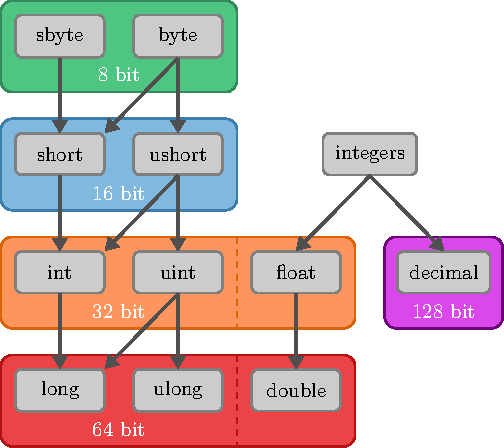
\includegraphics[height = 8cm, keepaspectratio = true]{figures/implicit_conversions.pdf}
    \caption{Numeric type implicit conversions in C\#.}
    % \label{}
\end{figure}
For example
\begin{lstlisting}
$ // 8 bit unsigned integer to 64 bit signed integer 
$ byte b = 32; Console.WriteLine($"{b} -- {b.GetType()}")
32 -- System.Byte
$ long l = b; Console.WriteLine($"{l} -- {l.GetType()}")
32 -- System.Int64

$ // 16 bit signed integer to double precision floating-point number
$ short s = 30000; Console.WriteLine($"{s} -- {s.GetType()}")
30000 -- System.Int16
$ double d = s; Console.WriteLine($"{d} -- {d.GetType()}")
30000 -- System.Double
\end{lstlisting}
\subsubsection{Explicit Conversion}
When a conversion cannot be made without risking losing information,
the compiler requires that we perform an explicit conversion using a \textbf{type cast}.
The syntax for a type cast is as follows
\begin{lstlisting}
(NEW_TYPE) EXPRESSION
\end{lstlisting}
For example
\begin{lstlisting}
$ // Decimal to single precision floating-point number
$ decimal pi = 3.14159265358979323m; Console.WriteLine($"{pi} -- {pi.GetType()}")
3.14159265358979323 -- System.Decimal
$ float fPi = (float) pi; Console.WriteLine($"{fPi} -- {fPi.GetType()}")
3.141593 -- System.Single

$ // 32 bit unsigned integer to 8 bit signed integer
$ uint u = 9876; Console.WriteLine($"{u} -- {u.GetType()}")
9876 -- System.UInt32
$ byte b = (byte) u; Console.WriteLine($"{b} -- {b.GetType()}")
148 -- System.Byte
\end{lstlisting}
In the final example, to understand what is happening in the explicit conversion,
we must look at the binary representation of the two integers.
\begin{lstlisting}
$ uint u = 9876; Console.WriteLine(Convert.ToString(u, 2).PadLeft(32, '0'))
00000000000000000010011010010100
$ byte b = (byte) u; Console.WriteLine(Convert.ToString(b, 2).PadLeft(8, '0'))
10010100
\end{lstlisting}
Notice that the value is determined by copying the 8 least significant bits
from the 32 bit unsigned integer.
\subsection{Operators}
The following table lists the C\texttt{\#} operators starting with the highest precedence to the lowest.
\begin{table}[H]
    \centering
    \begin{tabular}{>{\centering}p{0.45\linewidth} c}
        \toprule
        \textbf{Operators}                                                                                           & \textbf{Category}                 \\
        \midrule
        \lstinline!x.y!, \lstinline!f(x)!, \lstinline!a[i]!, \lstinline!x++!,
        \lstinline!x--!, \lstinline?x!?, \lstinline!x->y! and other keywords                                         & Primary                           \\
        \lstinline!+x!, \lstinline!-x!, \lstinline+!x+, \lstinline!~x!,
        \lstinline!++x!, \lstinline!--x!, \lstinline!^x!, \lstinline!(T)x!, \lstinline!await!,
        \lstinline!&x!, \lstinline!*x!, \lstinline!true!, \lstinline!false!                                          & Unary                             \\
        \lstinline!x..y!                                                                                             & Range                             \\
        \lstinline!switch!, \lstinline!with!                                                                         & ---                               \\
        \lstinline!x * y!, \lstinline!x / y!, \lstinline!x % y!                                                      & Multiplicative                    \\
        \lstinline!x + y!, \lstinline!x - y!                                                                         & Additive                          \\ % chktex 8
        \lstinline!x << y!, \lstinline!x >> y!                                                                       & Shift                             \\
        \lstinline!x < y!, \lstinline!x > y!, \lstinline!x <= y!, \lstinline!x >= y!, \lstinline!is!, \lstinline!as! & Relational and type-testing       \\
        \lstinline!x == y!, \lstinline?x != y?                                                                       & Equality                          \\ % chktex 26
        \lstinline!x & y!                                                                                            & Logical {\ttfamily{AND}}          \\
        \lstinline!x ^ y!                                                                                            & Logical {\ttfamily{XOR}}          \\
        \lstinline!x | y!                                                                                            & Logical {\ttfamily{OR}}           \\
        \lstinline!x && y!                                                                                           & Conditional {\ttfamily{AND}}      \\
        \lstinline!x || y!                                                                                           & Conditional {\ttfamily{OR}}       \\
        \lstinline!x ?? y!                                                                                           & Null-coalescing operator          \\ % chktex 26
        \lstinline!c ? t : f!                                                                                        & Conditional operator              \\ % chktex 26
        \lstinline!x = y!, \lstinline!=>! and shorthand assignments                                                  & Assignment and lambda declaration \\
        \bottomrule
    \end{tabular}
    \caption{Precedence of various operators in C\texttt{\#}.}
    % \label{}
\end{table}
In C\texttt{\#}, arithmetic operations behave as expected.
\begin{lstlisting}
$ 123 + 12
135 // System.Int32
$ 123 - 12
111 // System.Int32
$ 123 * 12
1476 // System.Int32
$ 123 / 12
10 // System.Int32
$ 123 % 12
3 // System.Int32
\end{lstlisting}
Binary operators always convert the resulting data type to the data type of the
argument with the largest size in memory
(with a few exceptions when converting between floating-point types).
Hence division between two integers truncates any floating-point precision.
\begin{lstlisting}
$ 123 / 12
10 // System.Int32
$ 123.0 / 12
10.25 // System.Double
$ 123 / 12.0
10.25 // System.Double
$ 123.0 / 12.0
10.25 // System.Double
\end{lstlisting}
Caution should be used when dividing two numbers to avoid loss of precision.
\end{document}
